\documentclass[prd,floatfix,preprintnumbers,amsmath,amssymb,nofootinbib,superscriptaddress]{revtex4}
\usepackage{graphicx}% Include figure filesg
\usepackage{subfigure}

\def\pheq{\phantom{=}}
\newcommand{\Deqn}[1]{{Eq.~(\ref{#1})}}
\newcommand{\Deqns}[1]{{Eqs.~(\ref{#1})}}
\newcommand{\Ceqn}[1]{{Equation~(\ref{#1})}}
\newcommand{\Dfig}[1]{{Fig.~\ref{#1}}}
\newcommand{\beq}{\begin{equation}}
\newcommand{\eeq}{\end{equation}}
\newcommand{\bea}{\begin{eqnarray}}
\newcommand{\eea}{\end{eqnarray}}
\newcommand{\tr}{{\mathop{\mathrm{tr}}\nolimits}}

\begin{document}

\title{Practicum 5: The Hellings-Downs (HD) curve and the JHLM statistic }

\maketitle

In this exercise you will compute the JHLM (see Ref.~\cite{Jenet}) statistic for 
three pulsar timing residual data sets. Ref.~\cite{Jenet} is included in you materials.

With your materials you also have a file called SkyPositions.txt.  This file contains the right 
ascension ($0$-$2\pi$) and declination ($0$-$\pi$) in radians for 20 pulsars. 
You also have three sets of 20 files
with pulsar timing residuals (dataset1-1.txt to dataset1-20.txt, dataset2-1.txt to 
dataset2-20.txt, dataset3-1.txt to dataset3-20.txt). Each file contains 500 data points 
of equally spaced timing residuals that span 10 years. These files potentially contain
a gravitational wave signal (which is flat when expressed in terms of $\Omega$).

The idea here is to use Eq. (1), Eq. (3), and Eq. (4) of Ref.~\cite{Jenet} to make an 
estimate of the significance, which is $\rho \sqrt{N_p}$ [where $\rho$ is 
given in Eq. (4)]. If $M$ is the number of pulsars, $N_p=M(M-1)/2$ is the number of pulsar pairs. 

\vspace{0.3in}
Here's a suggestion on how to proceed:

\begin{itemize}

\item The practicum materials include a file (Practicum5.py) that loads in a data file with the sky locations of the pulsars.
You'll first need to add some code that computes 
the and stores the value of the Hellings-Downs curve (using Eq. (3)), along with the angular 
separation for each pulsar pair.  You'll need 
two loops over the number of pulsars to determine the angular separation and expected value 
of the HD curve for all pulsar pairs.

\item For now just focus on the first data set (you can copy and paste your code for data sets 
2 and 3 later once everything is working). The Practicum5.py code also reads in the dataset1 files 
for each of the pulsars. Add some code to Practicum5.py that 
computes and stores the correlation for each pulsar pair, i.e. Eq.~(1) of~\cite{Jenet}. 
Again, you'll just need add a couple of for loops over the number of pulsars.

\item At this point you can make a plot of the correlation vs. angular separation for your 
pulsar pairs (this plot is included in your materials, dataset1HD.pdf, which shows the 
correlation versus angular separation in radians). Do you think there are gravitational 
waves in this data?

\item You can now calculate the JHLM statistic Eq. (4) (which is also called the correlation or coherence, 
and you have code for this that you wrote for Practicum4) 
between the HD values you expected to get for each of your pairs and the ones that you actually found.
You'll need to first compute the mean of the HD values $\bar r$, the mean of the correlations 
$\bar \zeta$, and their standard deviations ($\sigma_r$, $\sigma_\zeta$).  

\item To calculate the significance you need to multiply your value of $\rho$ by $\sqrt{N_p}$

\item Once your code is working, copy and paste it and edit it to read data sets 2 and 3 and 
compute the significances.  The sky positions of the pulsars are the same. You're done coding now.

\item You should now have 3 values of the significance.  Using Figure 1 below estimate the value of $\Omega$
in each of the three data sets (note that your estimates of the significance are for a particular instance
of timing residuals, so you shouldn't expect perfect agreement with the expected significance curve). 
Examples of typical values of $\Omega$ (with flat spectra) are $0$-$10^{-6}$ for cosmic string scenarios, 
or around $10^{-14}$ for inflation.

\item Why do you think the expected significance curve flattens out at large values of $\Omega$?

\item If you have extra time, here's something you could do.  As you've learned earlier this 
week, timing residuals are produced by subtrating out a timing model from the TOAs. 
The largest effect is the subtraction of a quadratic, because it takes out the low frequencies 
where much of our signal is coming from. Try subtracting out quadratics from the data sets 
and see how that changes the significance.

\end{itemize}

\begin{figure}[h]
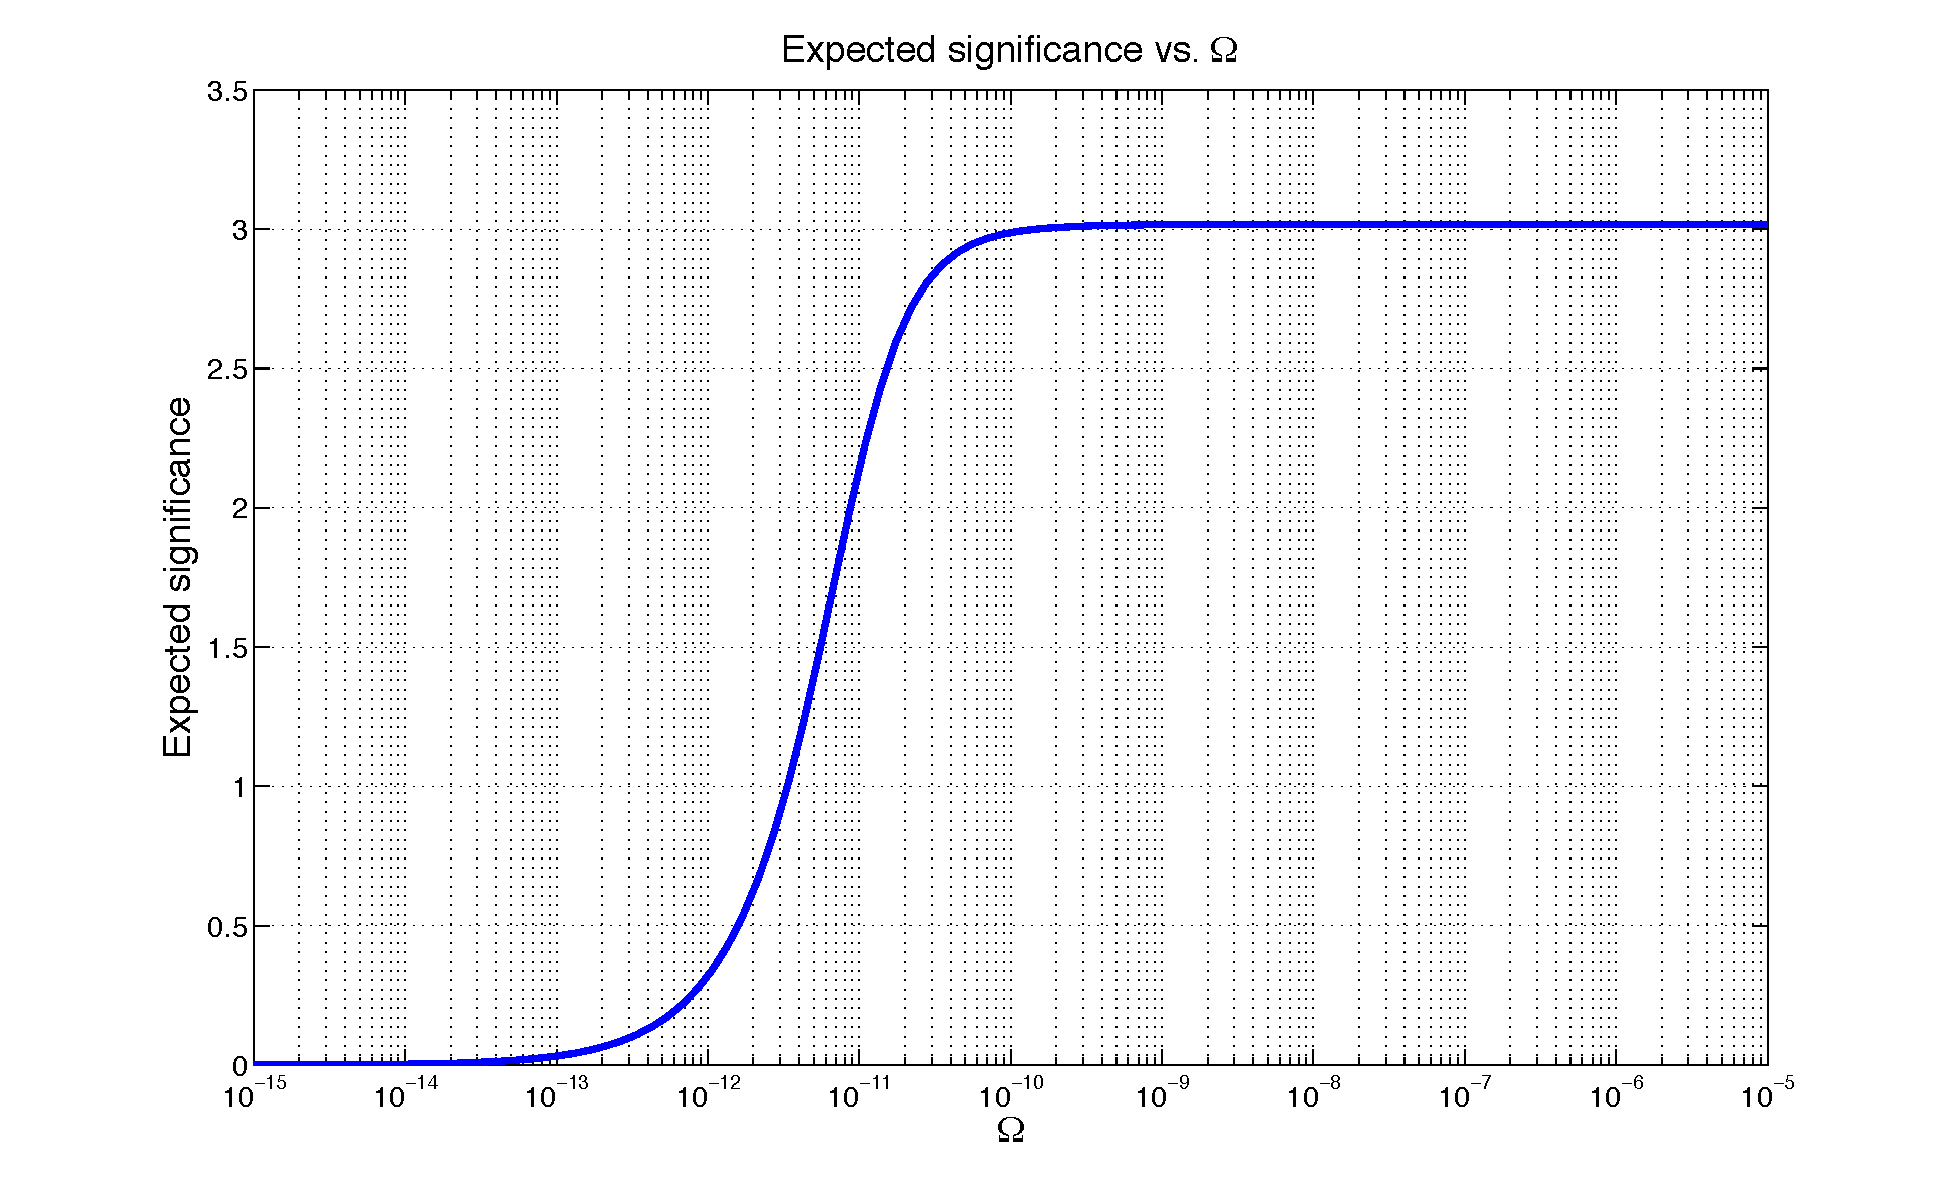
\includegraphics[width=20cm]{ExpectedSignificance}\\
\caption{Expected (average) significance versus $\Omega$ (flat spectrum).}
\end{figure}


\begin{thebibliography}{}

\bibitem{Jenet} Jenet et al.; ApJ. Letters 625, L123-L126 (2005).

\end{thebibliography}
\end{document}
